\documentclass[aspectratio=169]{beamer}
\usetheme{metropolis}
\usepackage{graphicx}
\usepackage{booktabs}
\usepackage{amsmath}
\usepackage[T1]{fontenc}
\usepackage[utf8]{inputenc}
\usepackage{tikz}
\graphicspath{{../results/figures/}}

\title{Dispersion, not displacement}
\subtitle{Loss of alveolar epithelial state coherence in lethal COVID-19}
\author{Pierce Taylor \& Chimdi Walter Ndubuisi \\ Computational Systems Biology 8190 \\ Dr.\ Toni Kazic}
\date{\today}

\begin{document}
\maketitle

% ---------------------------------------------------------------
\begin{frame}{The question in one sentence}
\Large
Do alveolar epithelial cells in lethal COVID-19 fail as a \alert{coherent block} (pushed toward one damaged state), or do they \alert{disperse} across many injury states?
\normalsize
\vspace{1em}
\begin{itemize}
  \item ``Coherent block'' $\Rightarrow$ expect \textbf{centroid displacement}.
  \item ``Dispersion'' $\Rightarrow$ expect \textbf{within-group variance inflation}.
  \item These predict \emph{opposite} things --- the failing test is informative.
\end{itemize}
\end{frame}

% ---------------------------------------------------------------
\begin{frame}{Why this matters}
\begin{itemize}
  \item Melms 2021, Delorey 2021 already described alveolar injury in COVID-19 lungs.
  \item Our contribution is \textbf{methodological}:
  \begin{itemize}
    \item Pre-specified geometric tests with opposing predictions
    \item 10 systematic ablations to separate robust from fragile findings
    \item Independent 618-donor cross-cohort replication
    \item Donor-level modeling, portable state scores, mechanistic decomposition
  \end{itemize}
  \item Honest reporting: which findings survive and which don't.
\end{itemize}
\end{frame}

% ---------------------------------------------------------------
\begin{frame}{Biology recap (for non-biologists)}
\begin{columns}[T]
\begin{column}{0.55\textwidth}
\textbf{Two cell types line each air sac:}
\begin{itemize}
  \item \textbf{AT1}: thin, flat, gas exchange ($\sim$95\% of surface)
  \item \textbf{AT2}: secrete surfactant + serve as local stem cells
\end{itemize}
\vspace{0.5em}
\textbf{When AT1 die:} AT2 $\to$ transitional (DATP) $\to$ AT1
\vspace{0.5em}
\textbf{In lethal COVID-19:}
\begin{itemize}
  \item SARS-CoV-2 enters AT2 via ACE2
  \item Kills both surfactant factory AND stem cells
  \item Transitional cells accumulate (stuck mid-repair)
\end{itemize}
\end{column}
\begin{column}{0.42\textwidth}
\small
\textbf{Key terms:}\\[3pt]
\textbf{snRNA-seq}: measure gene expression per nucleus\\[3pt]
\textbf{Pseudotime}: computational ordering along a biological process\\[3pt]
\textbf{Dispersion}: how spread out cells are in gene-expression space\\[3pt]
\textbf{DATP}: damage-associated transient progenitor (stuck mid-transition)
\end{column}
\end{columns}
\end{frame}

% ---------------------------------------------------------------
\begin{frame}{Data}
\begin{columns}[T]
\begin{column}{0.48\textwidth}
\textbf{Primary atlas (Melms 2021)}
\begin{itemize}
  \item SCP1219: 116{,}313 snRNA-seq nuclei
  \item 22{,}128 alveolar epithelial cells
  \item 7 healthy + 20 COVID-19 donors
  \item Full transcriptome ($\sim$20{,}000 genes)
\end{itemize}
\end{column}
\begin{column}{0.48\textwidth}
\textbf{Replication (cellxgene census)}
\begin{itemize}
  \item 89{,}736 AT1/AT2 cells
  \item 618 donors, 35 datasets
  \item SCP1219 \alert{excluded by ID}
  \item 84-gene panel only
\end{itemize}
\end{column}
\end{columns}
\vspace{0.8em}
\alert{True sample size: 27 donors, not 22{,}128 cells.}
\end{frame}

% ---------------------------------------------------------------
\begin{frame}{Pipeline at a glance}
\small
\begin{enumerate}
  \item QC: filter cells by gene count, mito \%
  \item Subset to alveolar epithelium (AT1 + AT2 + transitional)
  \item Normalize (10{,}000 counts/cell) $\to$ $\log(1+x)$
  \item 3{,}000 HVGs (Seurat v3) $\to$ Scale $\to$ 50-PC PCA
  \item $k$-NN ($k{=}15$) $\to$ UMAP + 15-component diffusion map
  \item Diffusion pseudotime rooted at healthy-AT2 centroid, normalized to $[0,1]$
  \item 8 curated gene programs scored via \texttt{sc.tl.score\_genes}
  \item 3 pre-specified statistical tests + 10 ablations
\end{enumerate}
\normalsize
Software: Python 3.12.3, Scanpy 1.12.1, seed 42.
\end{frame}

% ---------------------------------------------------------------
\begin{frame}{The manifold}
\centering
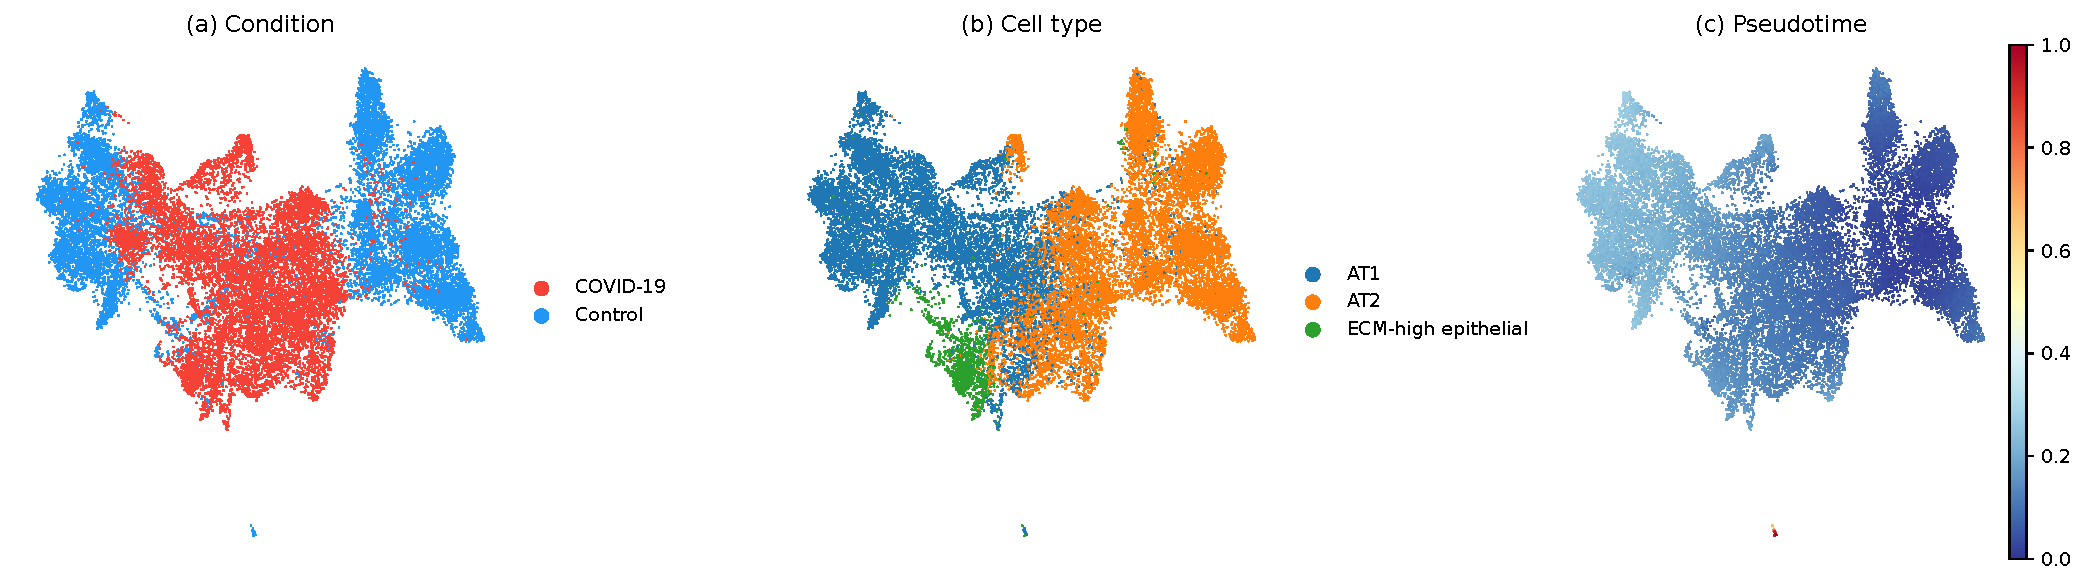
\includegraphics[width=0.95\linewidth]{fig2_manifold.pdf}
\\[3pt]
{\small UMAP colored by condition (left), cell type (center), pseudotime (right).}
\end{frame}

% ---------------------------------------------------------------
\begin{frame}{Result 1: Dispersion --- \textbf{the main finding}}
\begin{columns}[T]
\begin{column}{0.55\textwidth}
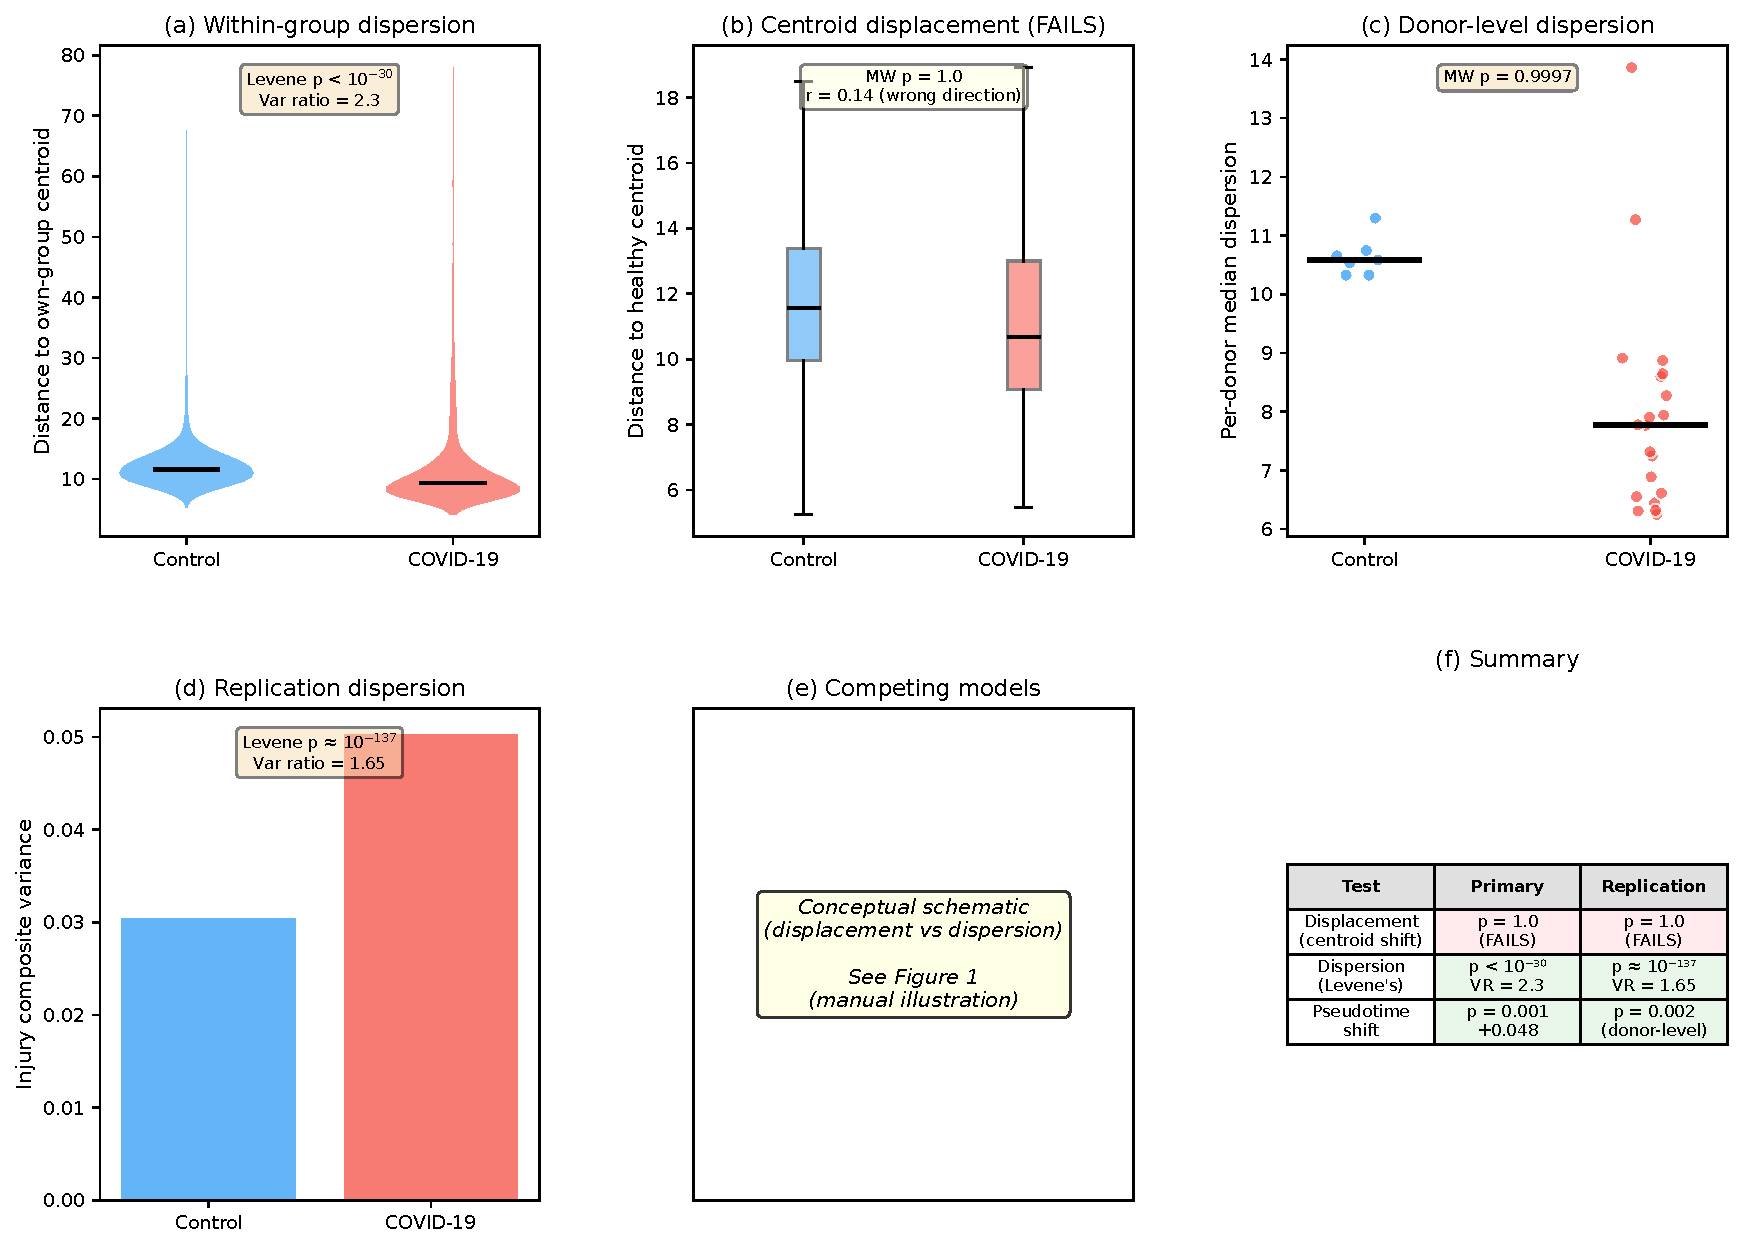
\includegraphics[width=\linewidth]{fig3_dispersion_centerpiece.pdf}
\end{column}
\begin{column}{0.42\textwidth}
\textbf{Within-group variance:}
\begin{itemize}
  \item COVID: 33.28
  \item Healthy: 14.58
  \item Ratio: \alert{2.3$\times$}
  \item Levene $p < 10^{-30}$
\end{itemize}
\vspace{0.5em}
COVID cells occupy a 2.3-fold broader region of gene-expression space.
\vspace{0.5em}
\alert{Replication}: ratio 1.65$\times$, $p \approx 10^{-137}$ across 618 donors.
\end{column}
\end{columns}
\end{frame}

% ---------------------------------------------------------------
\begin{frame}{Result 2: Centroid displacement \alert{fails}}
\begin{itemize}
  \item One-sided Mann--Whitney $U$ (COVID $>$ Healthy distance to healthy centroid): $p = \textbf{1.0}$
  \item COVID median distance: 10.68 \quad Healthy: 11.56
  \item COVID cells are actually \emph{closer} to the healthy centroid!
\end{itemize}
\vspace{0.5em}
\alert{This rules out the ``one coherent damaged state'' model.}
\vspace{0.5em}
Why? Some COVID cells stay near homeostatic identity while others scatter to distant positions. A mean-displacement test averages over both and sees nothing.
\end{frame}

% ---------------------------------------------------------------
\begin{frame}{Result 3: Pseudotime shift (supported)}
\begin{columns}[T]
\begin{column}{0.48\textwidth}
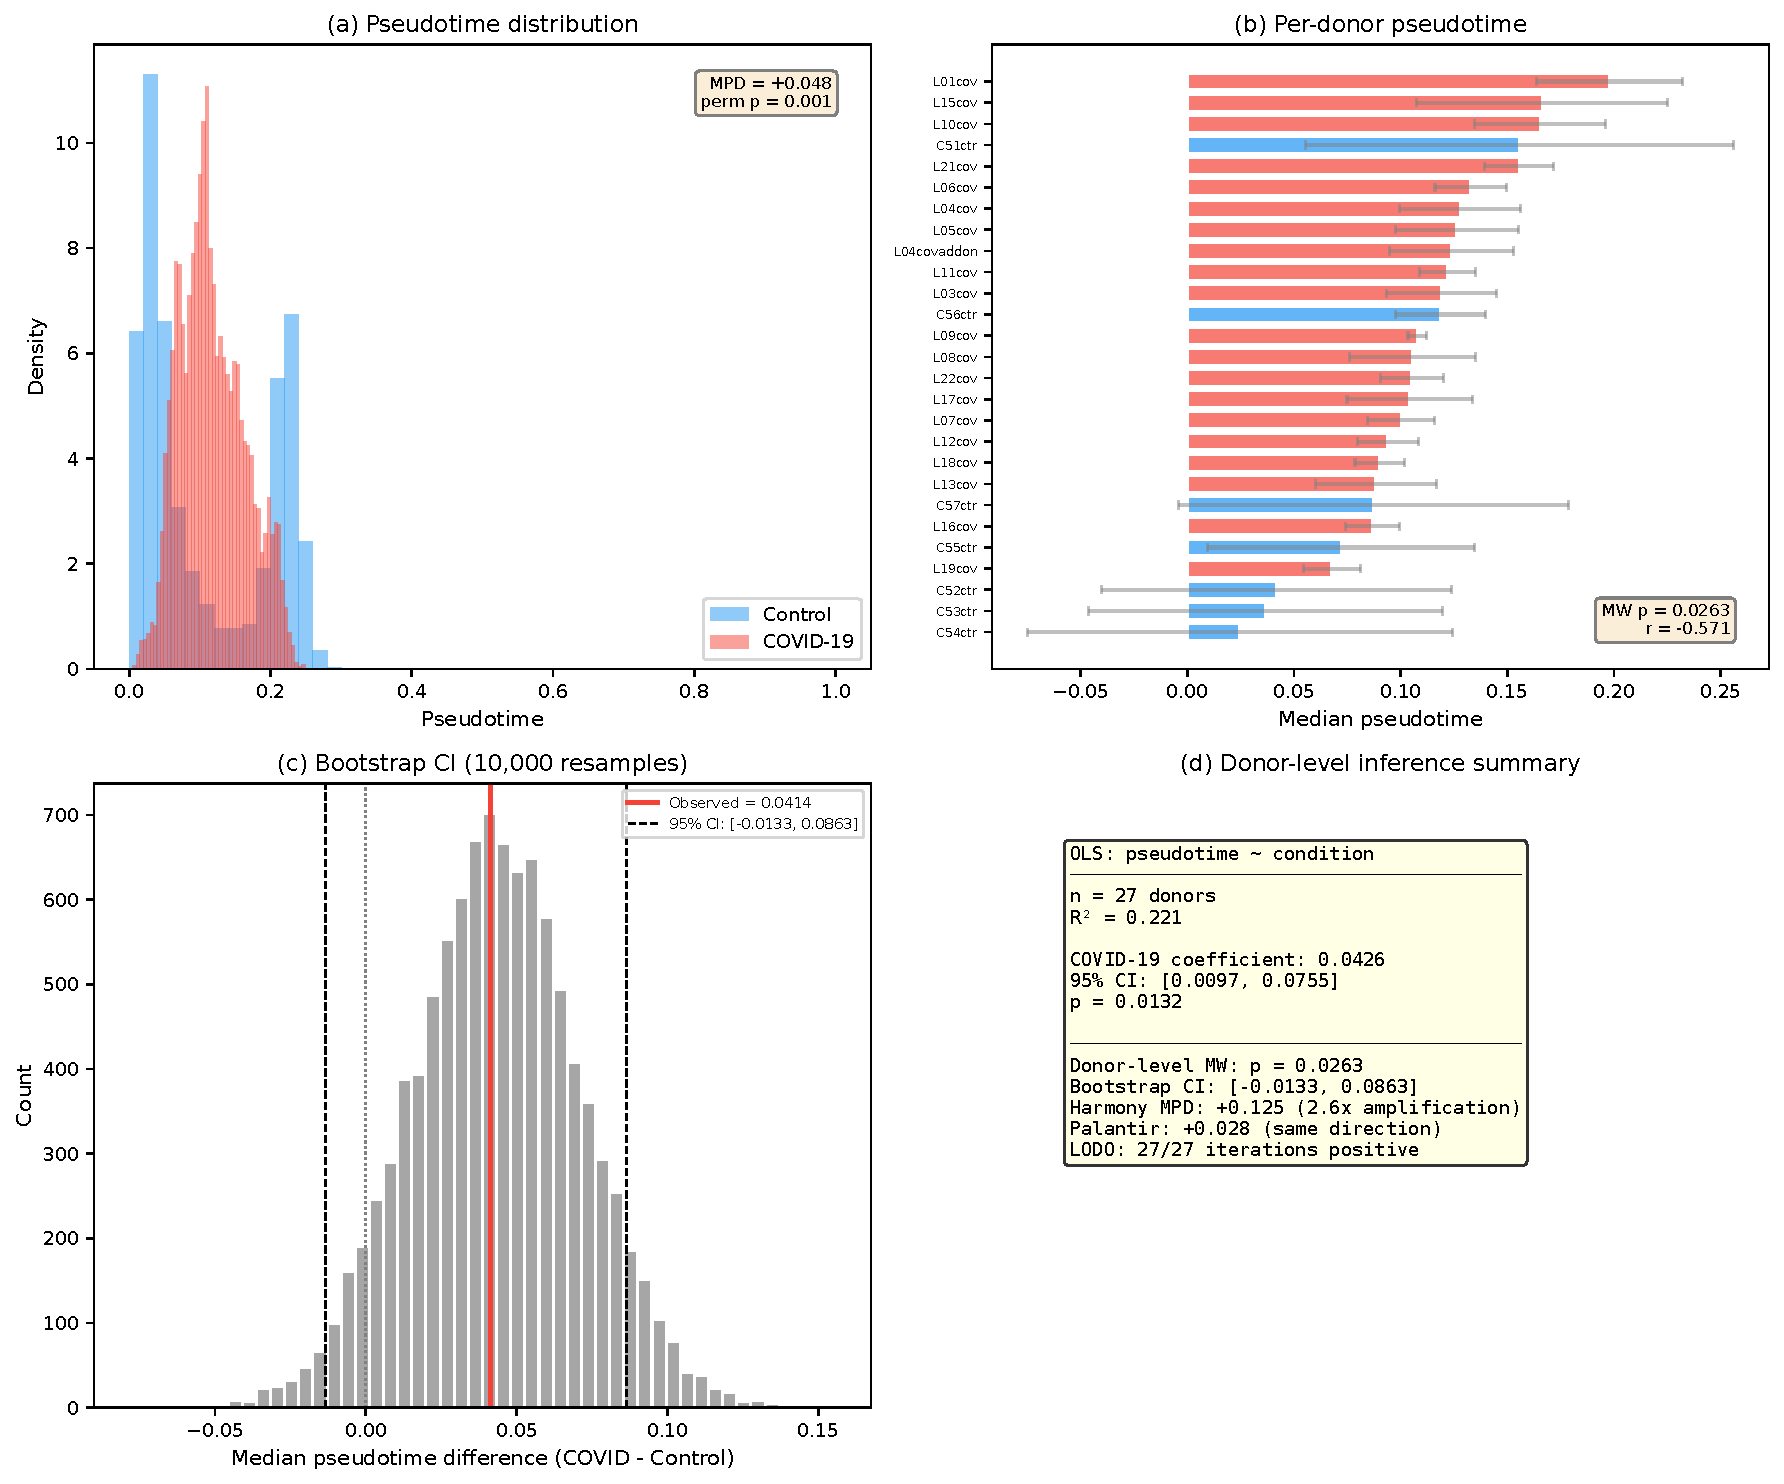
\includegraphics[width=\linewidth]{fig4_donor_pseudotime.pdf}
\end{column}
\begin{column}{0.48\textwidth}
\begin{itemize}
  \item Median: COVID 0.111 vs Healthy 0.063
  \item $\Delta = +0.048$ ($\sim$5\% of range)
  \item Permutation $p = 0.001$
  \item LOO: 27/27 donors preserve direction
  \item Harmony amplifies 2.6$\times$
\end{itemize}
\vspace{0.5em}
\textbf{Donor-level OLS:}\\
$\beta = +0.043$, $p = 0.013$, $R^2 = 0.22$
\end{column}
\end{columns}
\end{frame}

% ---------------------------------------------------------------
\begin{frame}{Donor-level dispersion: a surprising twist}
\begin{columns}[T]
\begin{column}{0.55\textwidth}
\textbf{Cell level:} COVID cells are 2.3$\times$ more dispersed.\\[6pt]
\textbf{Donor level:} COVID donors have \alert{lower} within-donor dispersion (7.77 vs 10.58).\\[6pt]
\textbf{Resolution:}\\
Individual COVID donors are \emph{not} internally messier. The cell-level dispersion arises because \alert{each COVID donor occupies a different region of injury space}.\\[6pt]
Pooling across donors creates apparent dispersion.
\end{column}
\begin{column}{0.42\textwidth}
\centering
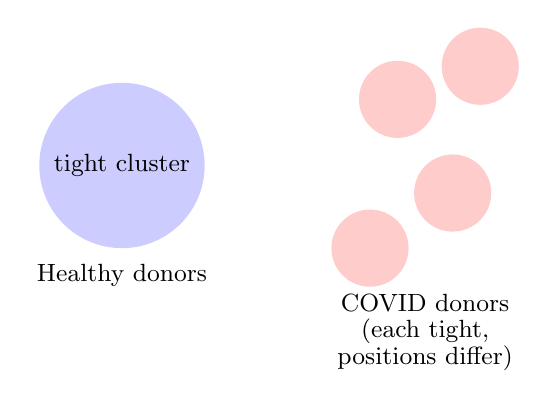
\begin{tikzpicture}[scale=0.7]
  % Healthy cluster
  \fill[blue!20] (0,0) circle (1.5);
  \node at (0,-2) {\small Healthy donors};
  \node at (0,0) {\small tight cluster};
  % COVID donors spread out
  \fill[red!20] (5,1.2) circle (0.7);
  \fill[red!20] (6,-0.5) circle (0.7);
  \fill[red!20] (4.5,-1.5) circle (0.7);
  \fill[red!20] (6.5,1.8) circle (0.7);
  \node at (5.5,-2.5) {\small COVID donors};
  \node at (5.5,-3) {\small (each tight,};
  \node at (5.5,-3.5) {\small positions differ)};
\end{tikzpicture}
\end{column}
\end{columns}
\end{frame}

% ---------------------------------------------------------------
\begin{frame}{Portable state scores}
\small
Marker-threshold DATP calling \alert{fails cross-cohort}. We developed 6 continuous scores:
\vspace{0.3em}
\begin{tabular}{llr}
\toprule
Score & What it measures & AUC (transitional) \\
\midrule
AT2 identity & Homeostatic AT2 markers & 0.323 \\
AT1 identity & Homeostatic AT1 markers & 0.375 \\
Transitional & KRT8/CLDN4/SFN markers & 0.441 \\
Injury composite & Mean of 6 injury programs & 0.630 \\
\alert{Coherence loss} & Distance from healthy centroid & \alert{0.972} \\
Repair failure & Transitional $-$ 0.5(AT2 + AT1) & 0.730 \\
\bottomrule
\end{tabular}
\normalsize
\vspace{0.5em}

All 6 scores: $p < 10^{-300}$ for condition separation in replication cohort.\\
\alert{Geometry-based scores transfer where marker thresholds fail.}
\end{frame}

% ---------------------------------------------------------------
\begin{frame}{Mechanistic decomposition: what drives the fan-out?}
\begin{columns}[T]
\begin{column}{0.48\textwidth}
\textbf{Which programs drive dispersion?}\\[6pt]
Linear regression: distance-to-healthy $\sim$ 8 programs\\
$R^2 = 0.115$\\[6pt]
\begin{tabular}{lr}
\toprule
Program & Coeff. \\
\midrule
Senescence & $+6.83$ \\
Oxidative stress & $+3.83$ \\
NF-$\kappa$B & $+1.95$ \\
AT2 identity & $-1.13$ \\
AT1 identity & $-1.02$ \\
\bottomrule
\end{tabular}
\end{column}
\begin{column}{0.48\textwidth}
\textbf{Interpretation:}\\[6pt]
The fan-out is driven by \alert{divergent activation of stress/senescence programs} across cells.\\[12pt]
Cells retaining homeostatic identity stay near the healthy centroid (negative coefficients).\\[12pt]
\textbf{Repair-stall:} COVID cells initiate repair but are diverted toward apoptosis rather than completing AT1 differentiation.
\end{column}
\end{columns}
\end{frame}

% ---------------------------------------------------------------
\begin{frame}{Transitional cells: enriched but not portable}
\begin{columns}[T]
\begin{column}{0.55\textwidth}
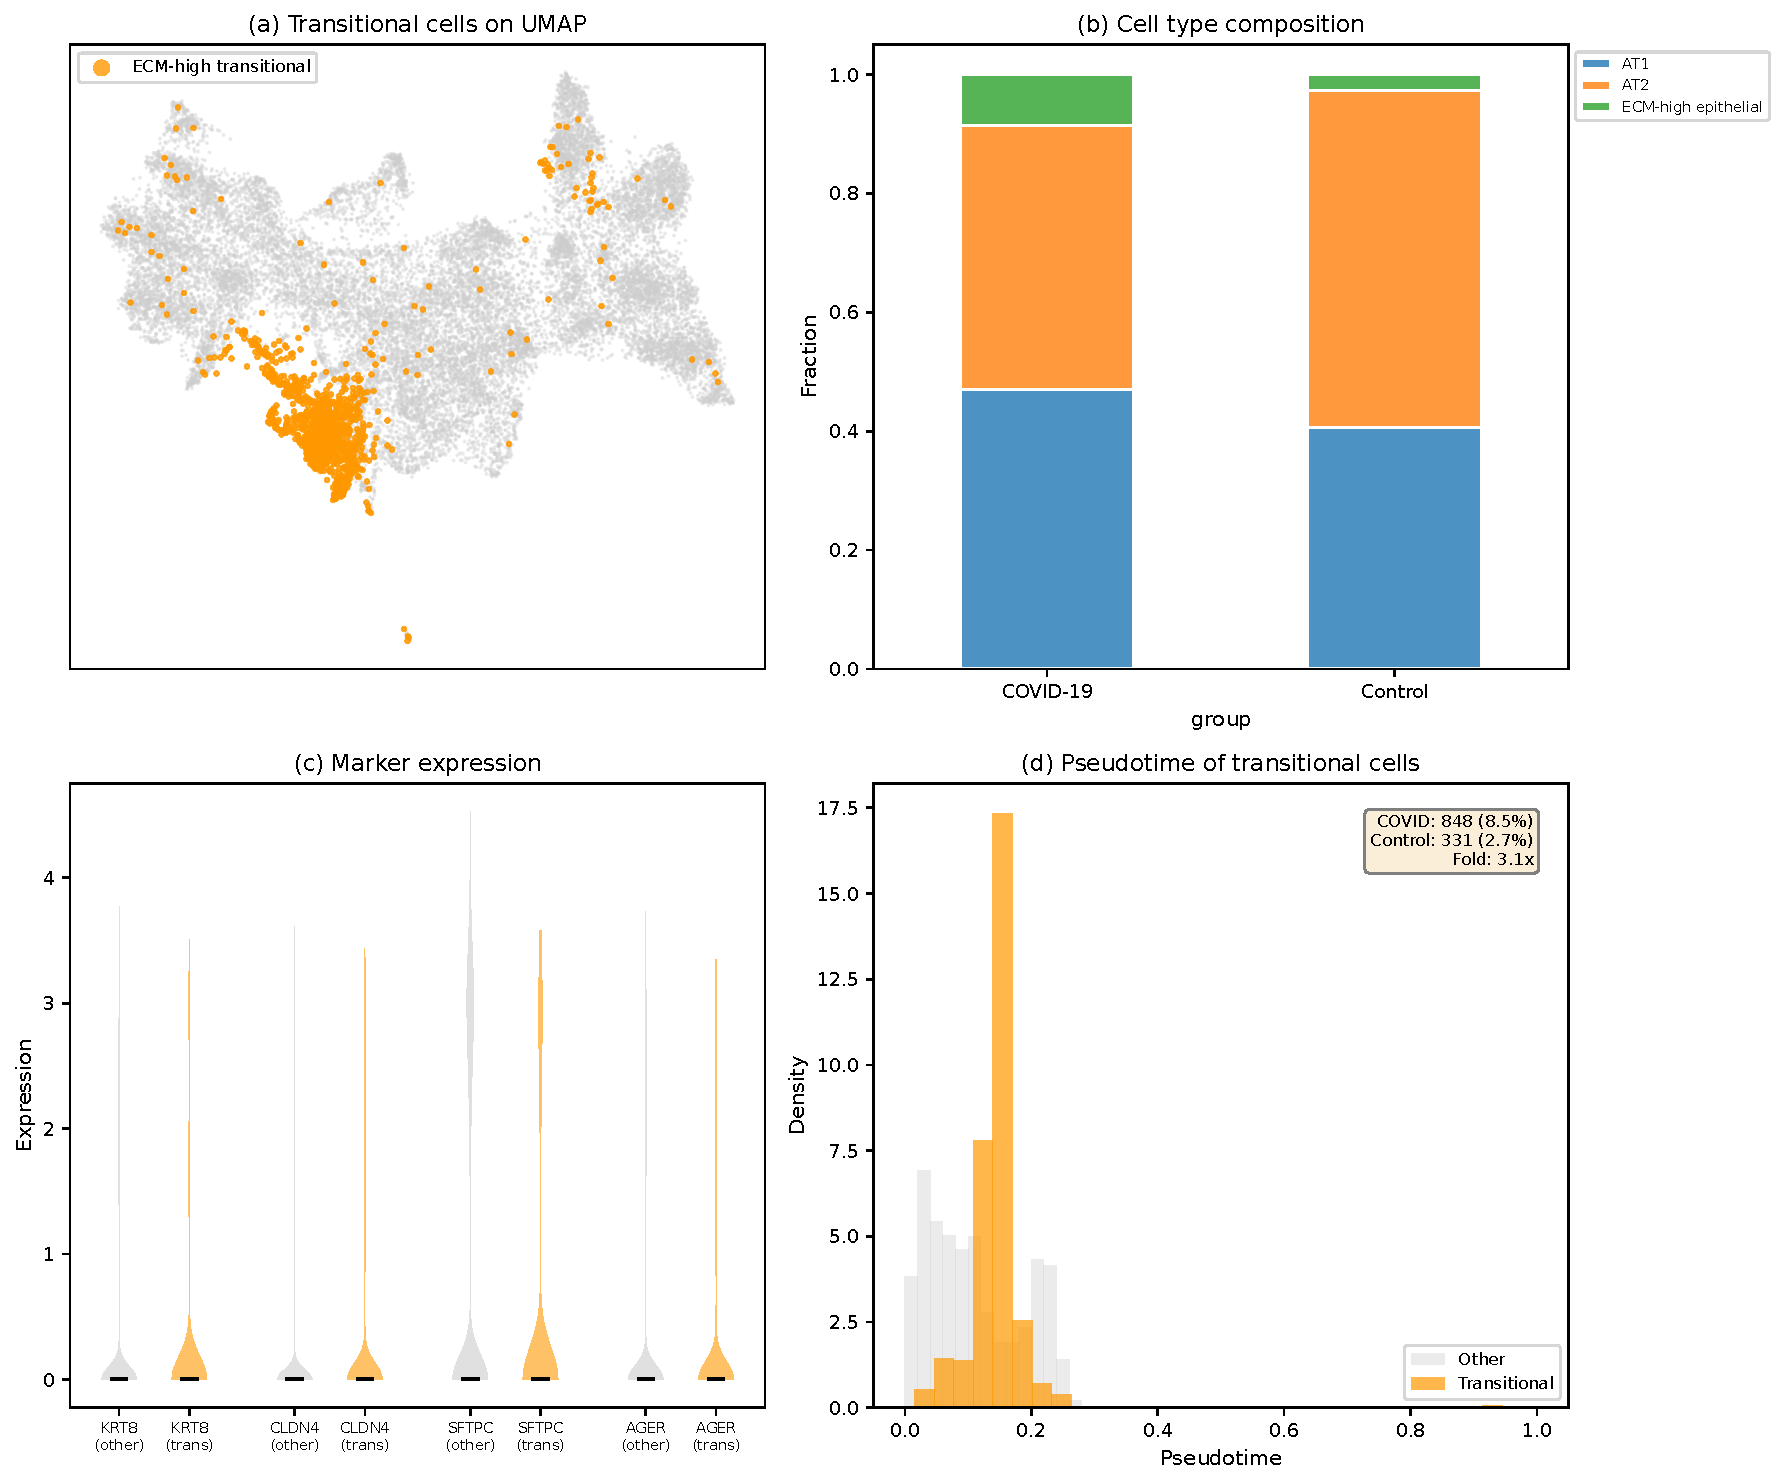
\includegraphics[width=\linewidth]{fig5_transitional.pdf}
\end{column}
\begin{column}{0.42\textwidth}
\textbf{Primary atlas:}\\
3.1$\times$ enriched in COVID (8.5\% vs 2.7\%)\\[6pt]
\alert{Replication:}\\
KRT8$^+$/CLDN4$^+$ threshold gives \emph{opposite} direction (0.48$\times$)\\[6pt]
\textbf{Lesson:} Marker-threshold cell-state definitions don't transfer across cohorts. Use manifold-based or classifier-based approaches.
\end{column}
\end{columns}
\end{frame}

% ---------------------------------------------------------------
\begin{frame}{Ten ablations --- stress testing robustness}
\centering
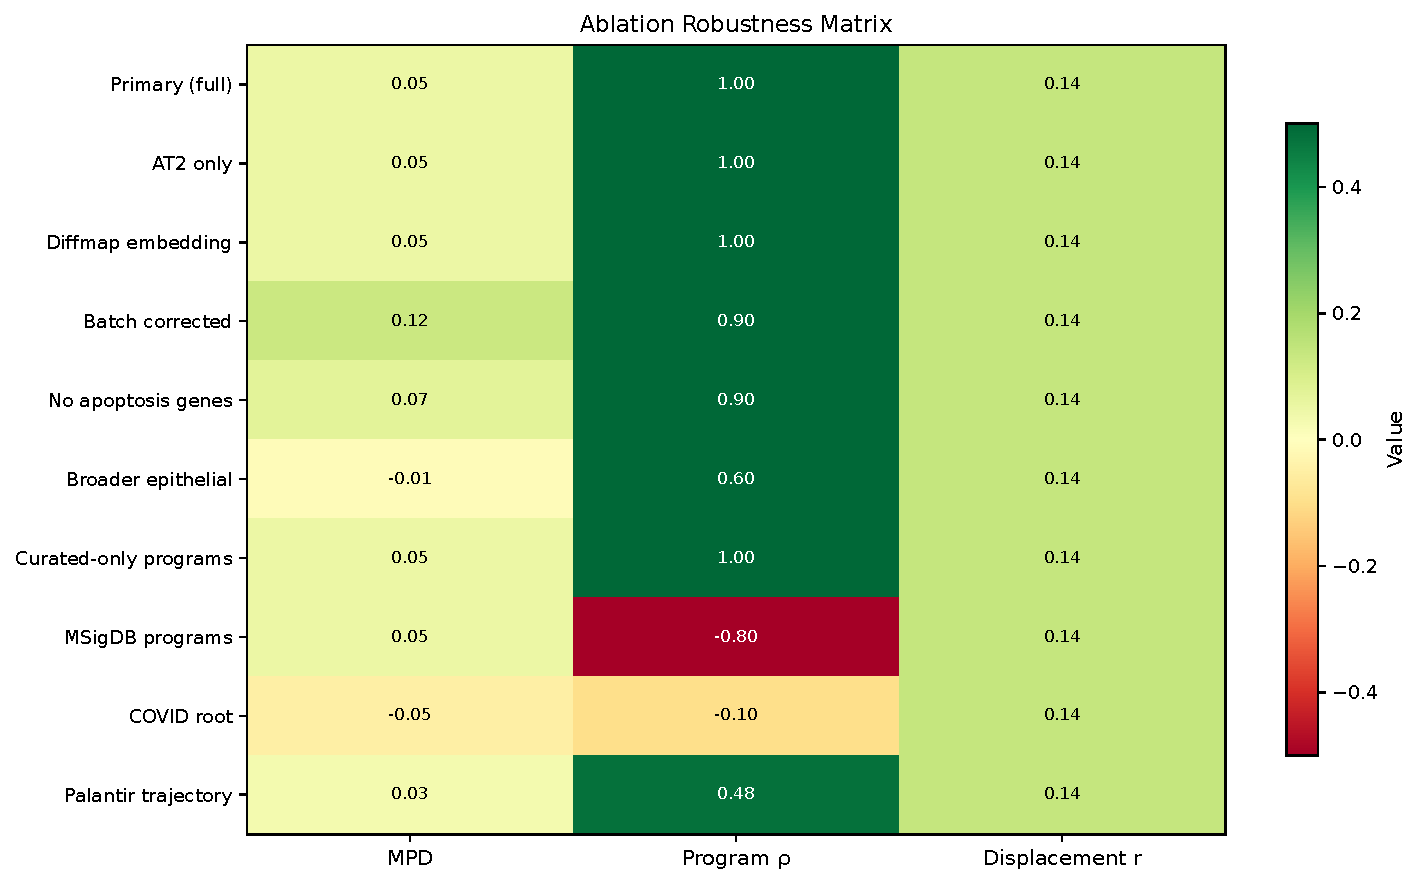
\includegraphics[width=0.85\linewidth]{fig6_ablation_matrix.pdf}
\\[3pt]
{\small Dispersion and pseudotime direction: \textbf{robust}. Fine program ordering: \textbf{fragile}.}
\end{frame}

% ---------------------------------------------------------------
\begin{frame}{The Harmony bug --- worth a slide}
\begin{itemize}
  \item Initially, corrected PCs were written with wrong orientation\\
        (PyTorch backend: cells$\times$PCs; old CPU backend: PCs$\times$cells)
  \item One-line fix: check shape and transpose if needed
  \item Post-fix: MPD $+0.048 \to +0.125$ (\textbf{2.6$\times$ amplification})
  \item Moral: ``batch correction didn't help'' can mean \emph{the pipeline is broken}, not \emph{the method doesn't matter}
\end{itemize}
\end{frame}

% ---------------------------------------------------------------
\begin{frame}{Independent replication: what transfers?}
\small
\begin{tabular}{lll}
\toprule
Finding & Primary & Replication (618 donors) \\
\midrule
Dispersion (Levene) & $p < 10^{-30}$, ratio 2.3$\times$ & \textbf{$p \approx 10^{-137}$, ratio 1.65$\times$} \\
Pseudotime direction & perm.\ $p = 0.001$ & donor-level $p = 0.002$ \\
Centroid displacement & \alert{fails} ($p=1.0$) & \alert{fails} ($p=1.0$) \\
KRT8$^+$/CLDN4$^+$ DATP & $3.1\times$ enriched & \alert{$0.48\times$ --- reversed} \\
State scores (6) & all significant & \textbf{all $p < 10^{-300}$} \\
\bottomrule
\end{tabular}
\normalsize
\vspace{0.5em}
\alert{Geometric findings} (dispersion, donor-level direction) are portable.\\
\alert{Annotation-dependent} findings (marker thresholds, program ordering) are not.
\end{frame}

% ---------------------------------------------------------------
\begin{frame}{Summary of evidence}
\centering
\begin{tabular}{lcccc}
\toprule
& Primary & Ablations & Replication & Verdict \\
\midrule
Dispersion & $p < 10^{-30}$ & 10/10 robust & $p \approx 10^{-137}$ & \textbf{Strong} \\
Pseudotime shift & $p = 0.001$ & 27/27 LOO & donor $p = 0.002$ & \textbf{Robust} \\
Donor-level OLS & $p = 0.013$ & --- & --- & \textbf{Supported} \\
Centroid displacement & $p = 1.0$ & 10/10 fails & $p = 1.0$ & \textbf{Ruled out} \\
DATP threshold & $3.1\times$ & --- & reversed & \alert{Not portable} \\
Fine program order & varies & inverts & --- & \alert{Fragile} \\
\bottomrule
\end{tabular}
\end{frame}

% ---------------------------------------------------------------
\begin{frame}{The conclusion in one paragraph}
\large
Lethal COVID-19 does not push alveolar epithelial cells coherently away from the healthy state.

\vspace{0.5em}
It \alert{fans them outward} across heterogeneous injury states --- driven by divergent senescence, oxidative stress, and inflammatory programs --- while each donor's cells occupy a different region of injury space.

\vspace{0.5em}
The strongest, most portable finding is \textbf{within-group dispersion}, which replicates across 35 datasets and 618 donors.
\end{frame}

% ---------------------------------------------------------------
\begin{frame}{Key takeaways for computational systems biology}
\begin{enumerate}
  \item \textbf{Pre-register opposing hypotheses.} A failing test is informative.
  \item \textbf{Dispersion $>$ centroid displacement} for heterogeneous disease states.
  \item \textbf{Donor-level pseudobulk} beats cell-level tests ($n = 27$, not $n = 22{,}128$).
  \item \textbf{Continuous state scores} beat marker thresholds for cross-cohort transfer.
  \item \textbf{Ablations catch bugs.} The Harmony orientation fix is exhibit A.
  \item \textbf{Report honestly} what fails, not just what succeeds.
\end{enumerate}
\end{frame}

% ---------------------------------------------------------------
\begin{frame}{Limitations}
\begin{itemize}
  \item Post-mortem, lethal cases only (no mild/moderate COVID)
  \item 27 donors is small --- bootstrap CI marginally includes zero
  \item Pseudotime = ordering, not elapsed time
  \item 84-gene replication panel: too narrow for independent manifold
  \item Fine program ordering inverts under alternative gene lists
  \item DATP marker thresholds don't transfer cross-cohort
  \item Post-mortem effects may confound stress/apoptosis programs
\end{itemize}
\end{frame}

% ---------------------------------------------------------------
\begin{frame}[standout]
Thank you. \\ Questions?
\end{frame}

\end{document}
